\documentclass[10pt, a4paper]{article}


\usepackage{wrapfig}
\usepackage{graphicx}
\usepackage[T1]{fontenc}
\usepackage[polish]{babel}
\usepackage[utf8]{inputenc}
\usepackage[font=footnotesize, labelfont=bf]{caption}
\usepackage{csquotes}
\usepackage{placeins}
\usepackage{booktabs}
\usepackage{siunitx}
\usepackage{amsmath}
\usepackage[margin=1in]{geometry}


\usepackage[backend=biber, sorting=ynt]{biblatex}
\addbibresource{draft.bib}

\newcommand{\code}[1]{\texttt{#1}}


\title{Bibliography
management:
\texttt{biblatex}
package}


\author{Krzytsztof
Wiśniewski}
\date{
}


\begin{document}
  \begin{titlepage}
    \centering


    \Large \textbf{UNIWERSYTET GDAŃSKI}\\ \textbf{WYDZIAŁ MATEMATYKI, FIZYKI I
    INFORMATYKI}

    \vspace{2.5cm}


    \large \textbf{Krzysztof Wiśniewski}\\ \textbf{numer albumu: 274276}

    \vspace{1.5cm}
    \raggedright \small Kierunek studiów: Bioinformatyka\\ Specjalność: Ogólna

    \vspace{1.5cm}


    \centering
    \Large \textbf{Optymalizacja oprogramowania w języku Python do analizy stanów kwantowych.}

    \vfill


    \raggedleft \normalsize Praca licencjacka\\ wykonana\\ pod kierunkiem\\ dr hab.
    Marcin Wieśniak, prof. UG\\

    \vfill


    \centering
    \large Gdańsk 2023
  \end{titlepage}
  \newpage


  \tableofcontents
  \newpage


  \begin{sloppypar}
    \begin{abstract}
      W tej pracy przeprowadzam analizę efektywności metod optymalizacji czasu pracy programu
      CSSFinder służącego do detekcji splątania kwantowego. Podejmowane przeze mnie
      wysiłki skupiają się w głównej mierze na doborze lepszych narzędzi pozwalających
      na wydajniejsze prowadzenie dużych ilości obliczeń macierzowych. Rozważane będą skutki
      re-implementacji w języku Python z wykorzystaniem bibliotek NumPy\cite{NumPy_Article}\cite{NumPy_Doc},
      Numba\cite{Numba_Article}\cite{Numba_Doc}, Cython\cite{Cython_The_Best_Of_Both}\cite{Cython_Org}
      oraz re-implementacja w języku Rust\cite{Rust_Programming_Language} z
      wykorzystaniem skrzyni\footnote{ang. crate, określenie na bibliotekę-pakiet w ekosystemie
      języka Rust.}. Każda z implementacji została przetestowana na specjalnie dobranym
      zestawie danych, a wyniki są na bieżąco omawiane. Pod koniec podsumowuję wady i
      zalety poszczególnych rozwiązań i rozważam w jakich scenariuszach najlepiej się
      one sprawują.
    \end{abstract}

    \section{Wstęp}


    \subsection{Dlaczego Python?}


    Na przestrzeni ostatnich 20 lat język Python, stworzony przez Guido van Rossum,
    zanotował intensywny wzrost popularności. Pokazują to liczne zestawienia, w tym
    zestawienie najczęściej wykorzystywanych języków programowanie na GitHub'ie\cite{GitHub_Top_languages},
    w którym Python w roku 2022 zajął 2 miejsce, czy też zestawienie TIOBE Index\cite{TIOBE_Software_Index},
    uznające ten język za obecnie najbardziej rozpowszechniony pośród doświadczonych programistów
    (Maj 2023).

    \FloatBarrier
    \begin{figure}[ht]
      \centering
      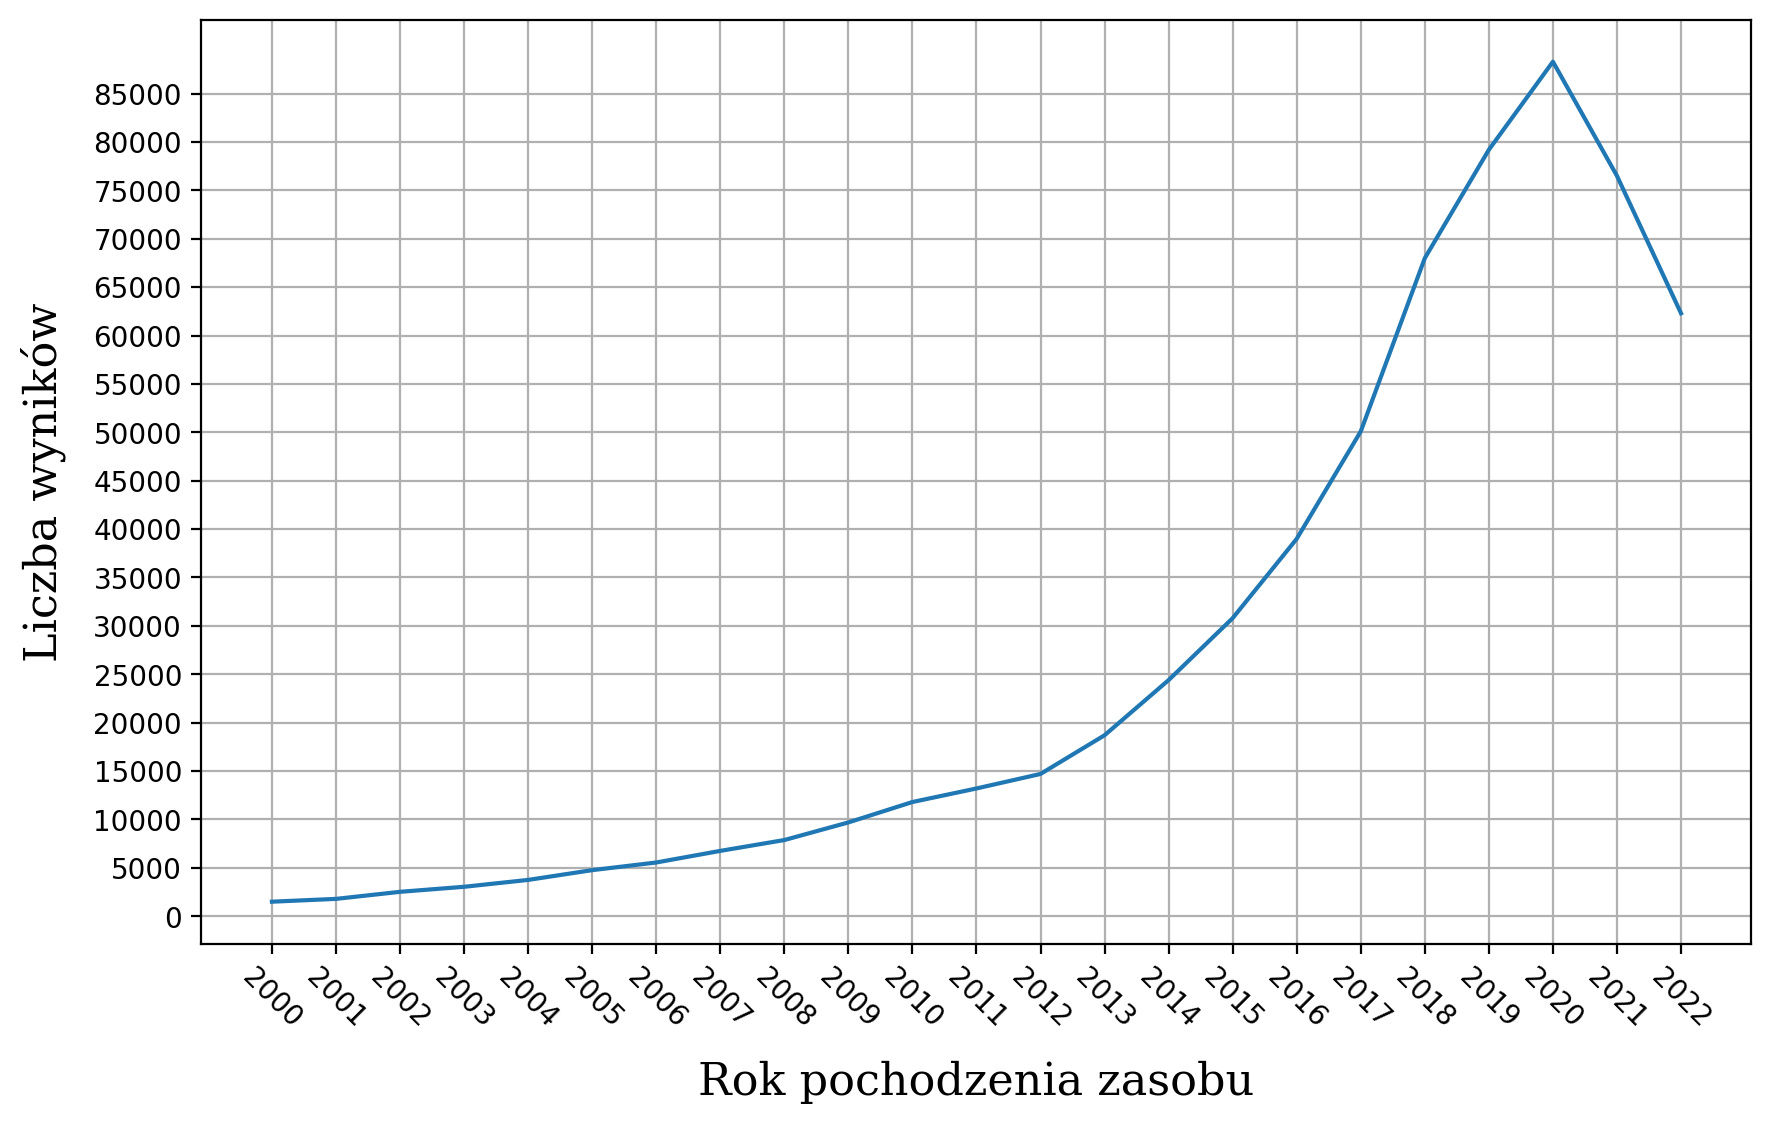
\includegraphics
      [width=0.75\textwidth]{"resources/images/python_language_results.png"}
      \caption{Ilość wyników zwróconych przez wyszukiwarkę Google Scholar dla zapytania 'python language' z podziałem na rok opublikowania zasobu w przestrzeni publicznej.}
    \end{figure}
    \FloatBarrier

    Niestety, interpretowany kod, napisany w Pythonie, pomimo licznych zalet, posiada
    również dotkliwą wadę - pod względem wydajności znacząco odstaje od kompilowanych
    języków programowania (C\cite{C_vs_Python}, C++\cite{Cpp_vs_Python}, Rust\cite{Rust_vs_Python}).
    Jednak, podejmując odpowiednie wysiłki, możliwe jest aby programy, których kluczowa logika
    została napisana w języku Python, zbliżały się wydajnością do odpowiedników
    przetłumaczonych na kod maszynowy. Taki stan rzeczy czyni z języka Python bardzo wygodny
    język do prototypownia w procesie wytwarzania nowych rozwiązań programistycznych.

    \subsection{Cel pracy}


    Praca ta ma na celu eksplorację wybranych metod optymalizacji czasu wykonania oprogramowania
    CSSFinder oraz weryfikację uzyskanych zmian wydajności programu. W dalszej jej
    części zaprezentuję wyniki testów wydajności i przeanalizuję specyfikę
    poszczególnych metod maksymalizacji wydajności. Podejście do redukcji czasu wykonywania
    programu zaprezentowane w tej pracy można zastosować dla większości oprogramowania,
    napisanego w języku Python, które koncentruje się na wykonywaniu dużych ilości obliczeń
    macierzowych.

    Do przeprowadzenia takich analiz konieczne było wielokrotne re-implementowanie części
    obliczeniowej programu. Funkcjonalny kod opisywany w tej pracy dostępny jest w
    repozytoriach Gita\cite{Git_Com} w serwisie GitHub \cite{CSSFinder_New}\cite{CSSFinder_New_Numpy}\cite{CSSFinder_New_Rust}.
    W skutek prac projektowych utworzona została również grupa publicznych pakietów, które
    można pobrać z serwisu PyPI:

    \begin{itemize}
      \item cssfinder\cite{CSSFinder_New_PyPI}

      \item cssfinder\_backend\_numpy\cite{CSSFinder_New_Numpy_PyPI}

      \item cssfinder\_backend\_rust\cite{CSSFinder_New_Rust_PyPI}
    \end{itemize}

    Zainstalowanie ich jest możliwe przy pomocy menadżera pakietów języka Python, np.
    \code{pip}\cite{PIP}. Pakiety są kompatybilne z implementacją CPython w wersjach 3.8
    - 3.10 i były testowane na systemach Windows (10), Linux (Ubuntu 22.04) oraz macOS (12).

    \subsection{Pochodzenie programu}


    Program CSSFinder, którego autorem jest dr hab. Marcin Wieśniak, prof. UG, z wydziału
    Matematyki, Fizyki i Informatyki Uniwersytetu Gdańskiego. Kod implementuje wyspecjalizowany
    wariant algorytmu zaproponowanego przez E. Gilberta\cite{Lindemann_Gilbert} który służy
    do znajdowania odległości pomiędzy punktem, a zbiorem wypukłym. Oprogramowanie jest przeznaczone
    do detekcji splątania kwantowego\cite{MW_Hilbert_Schmidt_distance}\cite{MW_Variational_approach}\cite{MW_Gilbert_Quantum_Entanglement}
    poprzez analizę macierzy gęstości opisujących układy kubitów\footnote{Potencjalnie również
    ku$d$itów, natomiast tego typu dane nie będą analizowane w tej pracy.}. Algorytm ten
    wielokrotnie, z sukcesem, był wykorzystany do analizy problemów z dziedziny fizyki kwantowej\cite{MW_Hilbert_Schmidt_distance}
    przy okazji również pokonując rozwiązania bazujące na uczeniu maszynowym\cite{MW_56_Year_Algorithm}.

    Oryginalna implementacja wykorzystuje język Python oraz bibliotekę NumPy. Posiada
    ona 4 różne tryby pracy, dedykowane do rozwiązywania różnych problemów, oznaczane
    kolejno cyframi:

    \begin{enumerate}
      \item pełna separowalność stanu $n$ ku$d$itów\footnote{ang. full separability of an
        $n$ qu$d$it state},

      \item separowalność stanu dwudzielnego\footnote{ang. separability of a bipartite state}

      \item rzeczywiste 3-częściowe uwikłanie stanu trzech ku$d$itów \footnote{genuine 3-partite
        entablement of a 3-quDit state}

      \item rzeczywiste 4-częściowe uwikłanie stanu trzech ku$d$itów \footnote{genuine 4-partite
        entablement of a 3-quDit state}
    \end{enumerate}

    Dodatkowo pozwala na podanie macierzy symetrii oraz macierzy projekcji układu.

    \newpage


    \section{Metody}


    \subsection{Środowisko testowe}


    Wszystkie wyniki wydajności uzyskane zostały przy użyciu następującego środowiska testowego:

    \FloatBarrier
    \begin{table}[ht]
      \centering
      \begin{tabular}{llllll}
    \midrule\midrule
    OS              & Ubuntu 22.04.2 LTS 64-bit         \\
    Kernel          & 5.19.0-42-generic                 \\
    Python          & 3.10.6 64-bit                     \\
    NumPy           & 1.23.5                            \\
    Numba           & 0.56.4                            \\
    Cython          & 3.0.0b1                           \\
    GCC             & 11.3.0 64-bit                     \\
    Rust            & 1.68.2 64-bit                     \\\midrule
    CPU             & AMD Ryzen 9 7950X                 \\
    RAM             & 64GB DDR5 5600MHz CL40            \\
    DRIVE           & 512GB SSD GOODRAM CX400 (SATA)    \\\midrule
  \end{tabular}
    \end{table}
    \FloatBarrier

    \subsection{Wstępne profilowanie}


    Prace nad optymalizacją kodu rozpocząłem od wstępnego profilowania pracy programu w
    trybie 1 (full separability of an n-quDit state) przekazując układ 5 kubitów opisany
    macierzą $\rho_{0}$ (Macierz $32\times 32$ podwójnej precyzji zmiennoprzecinkowych liczb
    zespolonych).

    \FloatBarrier
    \begin{figure}[ht]
      \centering
      \setcounter{MaxMatrixCols}{33}
      \[
        \rho_{0}= \left[
        \begin{smallmatrix}
          0.25  & 0 & 0.25  & 0 & 0 & 0 & 0 & 0 & 0 & 0 & 0 & 0 & 0 & 0 & 0 & 0 & 0 & 0 & 0 & 0 & 0 & 0 & 0 & 0 & 0.25  & 0 & 0 & 0 & 0 & 0 & 0 & -0.25 \\
          0     & 0 & 0     & 0 & 0 & 0 & 0 & 0 & 0 & 0 & 0 & 0 & 0 & 0 & 0 & 0 & 0 & 0 & 0 & 0 & 0 & 0 & 0 & 0 & 0     & 0 & 0 & 0 & 0 & 0 & 0 & 0     \\
          0.25  & 0 & 0.25  & 0 & 0 & 0 & 0 & 0 & 0 & 0 & 0 & 0 & 0 & 0 & 0 & 0 & 0 & 0 & 0 & 0 & 0 & 0 & 0 & 0 & 0.25  & 0 & 0 & 0 & 0 & 0 & 0 & -0.25 \\
          0     & 0 & 0     & 0 & 0 & 0 & 0 & 0 & 0 & 0 & 0 & 0 & 0 & 0 & 0 & 0 & 0 & 0 & 0 & 0 & 0 & 0 & 0 & 0 & 0     & 0 & 0 & 0 & 0 & 0 & 0 & 0     \\
          0     & 0 & 0     & 0 & 0 & 0 & 0 & 0 & 0 & 0 & 0 & 0 & 0 & 0 & 0 & 0 & 0 & 0 & 0 & 0 & 0 & 0 & 0 & 0 & 0     & 0 & 0 & 0 & 0 & 0 & 0 & 0     \\
          0     & 0 & 0     & 0 & 0 & 0 & 0 & 0 & 0 & 0 & 0 & 0 & 0 & 0 & 0 & 0 & 0 & 0 & 0 & 0 & 0 & 0 & 0 & 0 & 0     & 0 & 0 & 0 & 0 & 0 & 0 & 0     \\
          0     & 0 & 0     & 0 & 0 & 0 & 0 & 0 & 0 & 0 & 0 & 0 & 0 & 0 & 0 & 0 & 0 & 0 & 0 & 0 & 0 & 0 & 0 & 0 & 0     & 0 & 0 & 0 & 0 & 0 & 0 & 0     \\
          0     & 0 & 0     & 0 & 0 & 0 & 0 & 0 & 0 & 0 & 0 & 0 & 0 & 0 & 0 & 0 & 0 & 0 & 0 & 0 & 0 & 0 & 0 & 0 & 0     & 0 & 0 & 0 & 0 & 0 & 0 & 0     \\
          0     & 0 & 0     & 0 & 0 & 0 & 0 & 0 & 0 & 0 & 0 & 0 & 0 & 0 & 0 & 0 & 0 & 0 & 0 & 0 & 0 & 0 & 0 & 0 & 0     & 0 & 0 & 0 & 0 & 0 & 0 & 0     \\
          0     & 0 & 0     & 0 & 0 & 0 & 0 & 0 & 0 & 0 & 0 & 0 & 0 & 0 & 0 & 0 & 0 & 0 & 0 & 0 & 0 & 0 & 0 & 0 & 0     & 0 & 0 & 0 & 0 & 0 & 0 & 0     \\
          0     & 0 & 0     & 0 & 0 & 0 & 0 & 0 & 0 & 0 & 0 & 0 & 0 & 0 & 0 & 0 & 0 & 0 & 0 & 0 & 0 & 0 & 0 & 0 & 0     & 0 & 0 & 0 & 0 & 0 & 0 & 0     \\
          0     & 0 & 0     & 0 & 0 & 0 & 0 & 0 & 0 & 0 & 0 & 0 & 0 & 0 & 0 & 0 & 0 & 0 & 0 & 0 & 0 & 0 & 0 & 0 & 0     & 0 & 0 & 0 & 0 & 0 & 0 & 0     \\
          0     & 0 & 0     & 0 & 0 & 0 & 0 & 0 & 0 & 0 & 0 & 0 & 0 & 0 & 0 & 0 & 0 & 0 & 0 & 0 & 0 & 0 & 0 & 0 & 0     & 0 & 0 & 0 & 0 & 0 & 0 & 0     \\
          0     & 0 & 0     & 0 & 0 & 0 & 0 & 0 & 0 & 0 & 0 & 0 & 0 & 0 & 0 & 0 & 0 & 0 & 0 & 0 & 0 & 0 & 0 & 0 & 0     & 0 & 0 & 0 & 0 & 0 & 0 & 0     \\
          0     & 0 & 0     & 0 & 0 & 0 & 0 & 0 & 0 & 0 & 0 & 0 & 0 & 0 & 0 & 0 & 0 & 0 & 0 & 0 & 0 & 0 & 0 & 0 & 0     & 0 & 0 & 0 & 0 & 0 & 0 & 0     \\
          0     & 0 & 0     & 0 & 0 & 0 & 0 & 0 & 0 & 0 & 0 & 0 & 0 & 0 & 0 & 0 & 0 & 0 & 0 & 0 & 0 & 0 & 0 & 0 & 0     & 0 & 0 & 0 & 0 & 0 & 0 & 0     \\
          0     & 0 & 0     & 0 & 0 & 0 & 0 & 0 & 0 & 0 & 0 & 0 & 0 & 0 & 0 & 0 & 0 & 0 & 0 & 0 & 0 & 0 & 0 & 0 & 0     & 0 & 0 & 0 & 0 & 0 & 0 & 0     \\
          0     & 0 & 0     & 0 & 0 & 0 & 0 & 0 & 0 & 0 & 0 & 0 & 0 & 0 & 0 & 0 & 0 & 0 & 0 & 0 & 0 & 0 & 0 & 0 & 0     & 0 & 0 & 0 & 0 & 0 & 0 & 0     \\
          0     & 0 & 0     & 0 & 0 & 0 & 0 & 0 & 0 & 0 & 0 & 0 & 0 & 0 & 0 & 0 & 0 & 0 & 0 & 0 & 0 & 0 & 0 & 0 & 0     & 0 & 0 & 0 & 0 & 0 & 0 & 0     \\
          0     & 0 & 0     & 0 & 0 & 0 & 0 & 0 & 0 & 0 & 0 & 0 & 0 & 0 & 0 & 0 & 0 & 0 & 0 & 0 & 0 & 0 & 0 & 0 & 0     & 0 & 0 & 0 & 0 & 0 & 0 & 0     \\
          0     & 0 & 0     & 0 & 0 & 0 & 0 & 0 & 0 & 0 & 0 & 0 & 0 & 0 & 0 & 0 & 0 & 0 & 0 & 0 & 0 & 0 & 0 & 0 & 0     & 0 & 0 & 0 & 0 & 0 & 0 & 0     \\
          0     & 0 & 0     & 0 & 0 & 0 & 0 & 0 & 0 & 0 & 0 & 0 & 0 & 0 & 0 & 0 & 0 & 0 & 0 & 0 & 0 & 0 & 0 & 0 & 0     & 0 & 0 & 0 & 0 & 0 & 0 & 0     \\
          0     & 0 & 0     & 0 & 0 & 0 & 0 & 0 & 0 & 0 & 0 & 0 & 0 & 0 & 0 & 0 & 0 & 0 & 0 & 0 & 0 & 0 & 0 & 0 & 0     & 0 & 0 & 0 & 0 & 0 & 0 & 0     \\
          0     & 0 & 0     & 0 & 0 & 0 & 0 & 0 & 0 & 0 & 0 & 0 & 0 & 0 & 0 & 0 & 0 & 0 & 0 & 0 & 0 & 0 & 0 & 0 & 0     & 0 & 0 & 0 & 0 & 0 & 0 & 0     \\
          0.25  & 0 & 0.25  & 0 & 0 & 0 & 0 & 0 & 0 & 0 & 0 & 0 & 0 & 0 & 0 & 0 & 0 & 0 & 0 & 0 & 0 & 0 & 0 & 0 & 0.25  & 0 & 0 & 0 & 0 & 0 & 0 & -0.25 \\
          0     & 0 & 0     & 0 & 0 & 0 & 0 & 0 & 0 & 0 & 0 & 0 & 0 & 0 & 0 & 0 & 0 & 0 & 0 & 0 & 0 & 0 & 0 & 0 & 0     & 0 & 0 & 0 & 0 & 0 & 0 & 0     \\
          0     & 0 & 0     & 0 & 0 & 0 & 0 & 0 & 0 & 0 & 0 & 0 & 0 & 0 & 0 & 0 & 0 & 0 & 0 & 0 & 0 & 0 & 0 & 0 & 0     & 0 & 0 & 0 & 0 & 0 & 0 & 0     \\
          0     & 0 & 0     & 0 & 0 & 0 & 0 & 0 & 0 & 0 & 0 & 0 & 0 & 0 & 0 & 0 & 0 & 0 & 0 & 0 & 0 & 0 & 0 & 0 & 0     & 0 & 0 & 0 & 0 & 0 & 0 & 0     \\
          0     & 0 & 0     & 0 & 0 & 0 & 0 & 0 & 0 & 0 & 0 & 0 & 0 & 0 & 0 & 0 & 0 & 0 & 0 & 0 & 0 & 0 & 0 & 0 & 0     & 0 & 0 & 0 & 0 & 0 & 0 & 0     \\
          0     & 0 & 0     & 0 & 0 & 0 & 0 & 0 & 0 & 0 & 0 & 0 & 0 & 0 & 0 & 0 & 0 & 0 & 0 & 0 & 0 & 0 & 0 & 0 & 0     & 0 & 0 & 0 & 0 & 0 & 0 & 0     \\
          0     & 0 & 0     & 0 & 0 & 0 & 0 & 0 & 0 & 0 & 0 & 0 & 0 & 0 & 0 & 0 & 0 & 0 & 0 & 0 & 0 & 0 & 0 & 0 & 0     & 0 & 0 & 0 & 0 & 0 & 0 & 0     \\
          -0.25 & 0 & -0.25 & 0 & 0 & 0 & 0 & 0 & 0 & 0 & 0 & 0 & 0 & 0 & 0 & 0 & 0 & 0 & 0 & 0 & 0 & 0 & 0 & 0 & -0.25 & 0 & 0 & 0 & 0 & 0 & 0 & 0.25  \\
        \end{smallmatrix}
        \right]
      \]
      \caption{Macierz $\rho_{0}$.}
      \label{rho-0}
    \end{figure}

    \FloatBarrier

    Program wykonywał proces analizy stanu aż do uzyskania 1000 korekcji. Do zbierania danych
    o pracy programy wykorzystałem moduł z biblioteki standardowej języka Python, \code{cProfile}.
    Przy analizie tak uzyskanych wyników posiłkowałem się wizualizacjami wykonanymi przy
    pomocy biblioteki snakeviz\cite{Snakeviz_PyPI}. Podczas testów, program wykorzystywał
    domyślny globalny generator liczb losowych biblioteki NumPy (PCG64\cite{NumpyDefaultGenerator})
    z ziarnem ustawionym na wartość 0.

    \FloatBarrier
    \begin{figure}[ht]
      \centering
      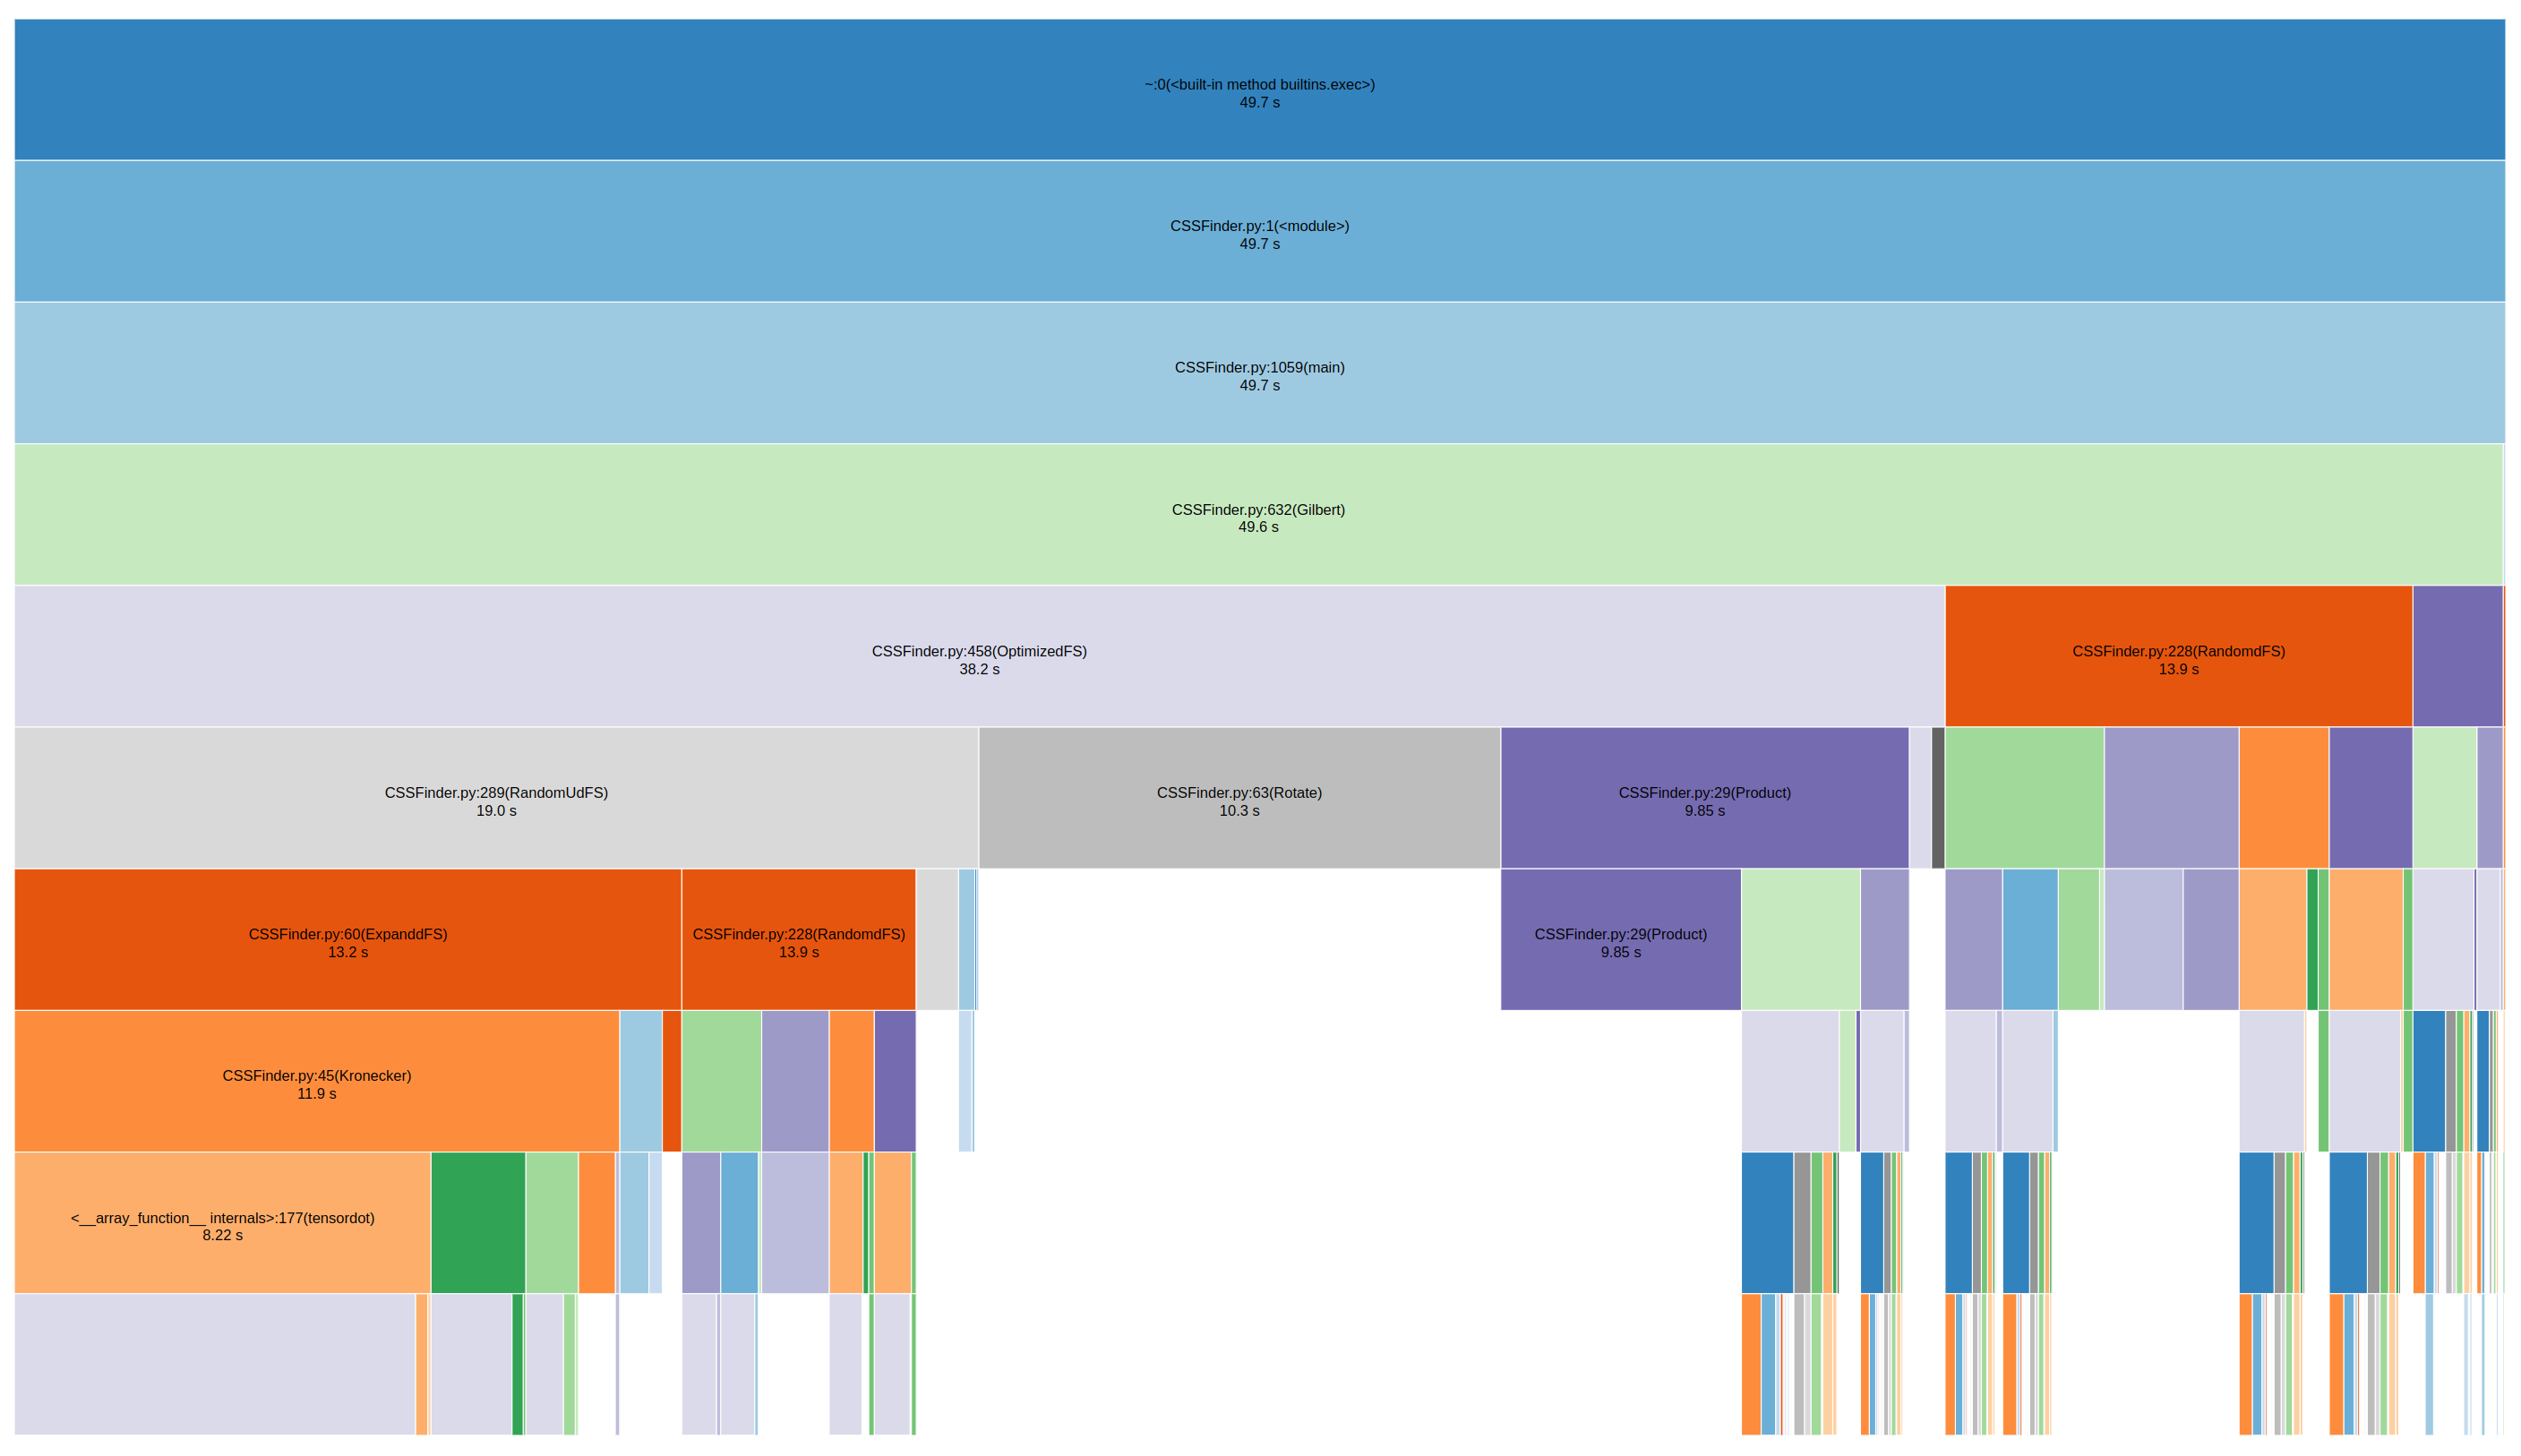
\includegraphics[width=1.0\textwidth]{"resources/profiling_1/graph.png"}
      \caption{Diagram podsumowujący pracę programu wygenerowany przez program snakeviz.}
      \label{pre-prof-perf}
    \end{figure}

    Rysunek \ref{pre-prof-perf} przedstawia diagram udziału poszczególnych funkcji w
    całkowitym czasie pracy programu. Pierwszy blok od góry to pierwsze wywołanie pochodzące
    z interpretera. Następnie bloki, których opisy zaczynają się od \code{CSSFinder.py}
    to wywołania w kodzie programu. Najniższe bloki to wywołania do funkcji bibliotek,
    głównie NumPy. \code{Snakeviz} automatycznie podejmuje decyzję o nie adnotowaniu
    bloku gdy opis nie ma szansy zmieścić się w obrębie bloku. Aby usunąć z diagramu zbędny
    szum informacyjny, funkcje których wykonywanie zajęło mniej niż 1\% czasu programu były
    pomijane.

    \FloatBarrier
    \begin{table}[ht]
      \tiny
      \centering
      \begin{tabular}{llllll}
  ncalls  & tottime   & percall   & cumtime   & percall   & filename:lineno(function)         \\
  \midrule\midrule
  1       & 1.431e-05 & 1.431e-05 & 49.72     & 49.72     & CSSFinder.py:1(\&lt;module\&gt;)  \\
  1       & 7.526e-05 & 7.526e-05 & 49.68     & 49.68     & CSSFinder.py:1059(main)           \\
  1       & 0.3098    & 0.3098    & 49.63     & 49.63     & CSSFinder.py:632(Gilbert)         \\
  1028    & 0.5381    & 0.0005234 & 38.2      & 0.03716   & CSSFinder.py:458(OptimizedFS)     \\\midrule
  411200  & 0.8332    & 2.026e-06 & 19.03     & 4.627e-05 & CSSFinder.py:289(RandomUdFS)      \\
  595516  & 0.67      & 1.125e-06 & 13.88     & 2.331e-05 & CSSFinder.py:228(RandomdFS)       \\
  411200  & 0.384     & 9.338e-07 & 13.17     & 3.203e-05 & CSSFinder.py:60(ExpanddFS)        \\
  822400  & 0.7256    & 8.823e-07 & 11.94     & 1.452e-05 & CSSFinder.py:45(Kronecker)        \\\midrule
  849257  & 10.3      & 1.213e-05 & 10.3      & 1.213e-05 & CSSFinder.py:63(Rotate)           \\
  1068026 & 6.535     & 6.118e-06 & 9.85      & 9.223e-06 & CSSFinder.py:29(Product)          \\
  1332780 & 2.17      & 1.628e-06 & 4.502     & 3.378e-06 & CSSFinder.py:21(Normalize)        \\
  1332780 & 2.247     & 1.686e-06 & 3.802     & 2.853e-06 & CSSFinder.py:33(Generate)         \\\midrule
  737264  & 0.4225    & 5.73e-07  & 2.548     & 3.456e-06 & CSSFinder.py:18(Outer)            \\
  595516  & 0.4642    & 7.794e-07 & 2.361     & 3.964e-06 & CSSFinder.py:26(Project)          \\
  1233601 & 0.8998    & 7.294e-07 & 1.165     & 9.447e-07 & CSSFinder.py:39(IdMatrix)         \\
  1       & 3.046e-06 & 3.046e-06 & 0.05277   & 0.05277   & CSSFinder.py:96(readmtx)          \\\midrule
  1       & 1.752e-06 & 1.752e-06 & 0.05277   & 0.05277   & CSSFinder.py:552(Initrho0)        \\
  1       & 4.597e-06 & 4.597e-06 & 0.002477  & 0.002477  & CSSFinder.py:1049(DisplayLogo)    \\
  1       & 5.189e-06 & 5.189e-06 & 0.0004394 & 0.0004394 & CSSFinder.py:954(DetectDim0)      \\
  1       & 1.628e-05 & 1.628e-05 & 2.526e-05 & 2.526e-05 & CSSFinder.py:556(Initrho1)        \\\midrule
  1       & 1.903e-06 & 1.903e-06 & 5.671e-06 & 5.671e-06 & CSSFinder.py:599(DefineSym)       \\
  40      & 3.038e-06 & 7.595e-08 & 3.038e-06 & 7.595e-08 & CSSFinder.py:192(writemtx)        \\
  1       & 1.102e-06 & 1.102e-06 & 2.846e-06 & 2.846e-06 & CSSFinder.py:624(DefineProj)      \\
  2       & 2.3e-07   & 1.15e-07  & 2.3e-07   & 1.15e-07  & CSSFinder.py:845(makeshortreport) \\\midrule
\end{tabular}
      \caption{{} Dane dotyczące pracy oryginalnej implementacji programu CSSFinder uzyskane przy pomocy programy cProfile. Tabela posiada oryginalne nazwy kolumn, nadane przez program \code{snakeviz}. Znaczenia kolumn, kolejno od lewej: \code{ncalls} - ilość wywołań funkcji. \code{tottime} - całkowity czas spędzony w ciele funkcji bez czasu spędzonego w wywołaniach do podfunkcji. \code{percall} - \code{totime} dzielone przez \code{ncalls}. \code{cumtime} - całkowity czas spędzony w wewnątrz funkcji i w wywołaniach podfunkcji. \code{percall} - \code{cumtime} dzielone przez \code{ncalls}. \code{filename:lineno(function)} - Plik, linia i nazwa funkcji.}
    \end{table}
    \FloatBarrier

    Z uzyskanych danych wynika że znakomitą większość (77\%\footnote{Wartość 77\% jak i
    wartości procentowe dalszej części tego akapitu zostały zaokrąglone do jedności, ze względu
    na małe znaczenie rzeczowe części ułamkowych.}) czasu pracy programu zajmuje funkcja
    \code{OptimizedFS()} . W jej wnętrzu 38\% czasu pochłania proces generowania
    losowych macierzy unitarnych, który w dużej mierze wykorzystuje mnożenia tensorowe (26\%).
    Poza funkcją \code{OptimizedFS()}, znaczący wpływ na czas wykonywania ma też funkcja
    `rotate()`, która pochłania około 21\% czasu działania programu. Kolejne 20\% czasu zajmuje
    funkcja \code{product()}, obliczająca odległość Hilberta-Schmidta pomiędzy dwoma stanami.
    Pozostałe wywołania mają stosunkowo marginalny wpływ na czas pracy i ich analiza na
    tym etapie nie niesie za sobą znaczących korzyści.

    Takie wyniki wskazują jednoznacznie że kluczowa dla czasu pracy programu jest tu
    maksymalizacja wydajności operacji macierzowych. Ten pozornie oczywisty wniosek wyznacza
    prosty kurs dalszych prac nad programem. W uzyskanych danych nie widać problemów z
    operacjami I/O\footnote{I/O - operacje wejścia wyjścia, w tym wypadku odczyt z i
    pisanie do plików.}, nie jest więc konieczne sięganie po rozwiązania takie jak asyncio
    czy wielowątkowość.

    \subsection{Wstępne pomiary wydajności}


    Aby uzyskać dobrą bazę porównawczą, wykonałem serię pomiarów czasu pracy programu na
    o różnych wymiarach macierzach gęstości. Reprezentowały one układy od 2 do 6 kubitów
    i przyjmowały rozmiary od $4\times4$ do $64\times64$. Przyjmowały one następującą
    postać:

    \[
      \rho_{n}=
      \begin{bmatrix}
        0.5    & 0      & \hdots & 0      & 0.5    \\
        0      & 0      & \hdots & 0      & 0      \\
        \vdots & \vdots &        & \vdots & \vdots \\
        0      & 0      & \hdots & 0      & 0      \\
        0.5    & 0      & \hdots & 0      & 0.5    \\
      \end{bmatrix}
    \]

    W dalszej części pracy wielokrotnie będę wykorzystywał tę grupę macierzy do testów wydajności.
    W tekście macierze te będą oznaczane jako $\rho_{2}$ do $\rho_{6}$, w zależności od reprezentowanej
    ilości kubitów\footnote{Tak więc macierz $\rho_{2}$ ma wymiary $4\times4$ i
    reprezentuje 2 kubity, macierz $\rho_{3}$ ma wymiary $8\times8$ i reprezentuje 3 kubity,
    macierz $\rho_{4}$ ma wymiary $16\times16$ i reprezentuje 4 kubity, itd. aż do
    $\rho_{6}$.}.

    Dane przekazywałem kolejno do programu z poleceniem działania w trybie 1 (full separability
    of an n-quDit state) do osiągnięcia 1000 korekcji lub do 2.000.000 iteracji algorytmu,
    w zależności od tego co nastąpi szybciej. Dla wszystkich macierzy algorytm uzyskał 1000
    korekcji i w żadnym przypadku nie osiągnął maksymalnej ilości iteracji. Dla każdej
    macierzy pomiar był powtarzany pięciokrotnie, a wyniki z pomiarów zostały uśrednione.
    Podczas obliczeń ziarno globalnego generatora liczb losowych biblioteki NumPy było
    ustawione na 0. Pomiary czasu pracy dotyczyły wyłącznie samego algorytmu\footnote{tj.
    funkcji `Gilbert()', nie biorą więc pod uwagę czasu pochłoniętego przez importowanie
    modułów, ładowanie danych itp. natomiast operacje pisania do plików które były wykonywane
    w obrębie tej funkcji są wliczane w czas pracy.}.

    \FloatBarrier
    \begin{figure}[ht]
      \centering
      \includegraphics[width=0.9\textwidth]{"resources/benchmark_1/plot.png"}
      \caption{Wyniki wstępnych testów wydajności oryginalnego kodu z zablokowaną (niebieski) i odblokowaną (pomarańczowy) liczbą wątków obliczeniowych dla macierzy $\rho
      _{2}$ - $\rho_{6}$.}
      \label{pre-perf}
    \end{figure}
    \FloatBarrier

    Podczas testów zaobserwowałem interesujące zjawisko dotyczące wydajności dla
    macierzy $64\times64$. W przypadku takich rozmiarów danych biblioteka NumPy automatycznie
    decyduje o wykorzystaniu wielowątkowej implementacji mnożenia macierzowego. Niestety,
    daje to efekt odwrotny do zamierzonego - obliczenia zamiast przyspieszać zwalniają.
    Na rysunku \ref{pre-perf} czasy obliczeń dla różnych rozmiarów macierzy z domyślnym
    zachowaniem biblioteki przedstawiają kolumny pomarańczowe. Jeśli przy pomocy zmiennych
    środowiskowych ustawimy ilość wątków wykorzystywanych do obliczeń na 1, co
    przedstawiają kolumny niebieskie, uzyskujemy znaczące skrócenie czasu obliczeń dla macierzy
    $64\times64$. Dla macierzy w mniejszych rozmiarach nie odnotowałem różnicy w
    wydajności pomiędzy konfiguracją domyślną, a manualnie dostosowywaną. Warto dodać że
    ilość iteracji wykonywanych przez program nie zmienia się, różnica wynika wyłącznie z
    czasu trwania operacji arytmetycznych. Taki stan rzeczy najprawdopodobniej jest
    wynikiem dodatkowego obciążenia ze strony komunikacji i/lub synchronizacji między
    wątkami.

    \subsection{Modularyzacja}


    Podczas procesu optymalizacji planowałem wypróbować liczne rozwiązania, które wymagały
    zasadniczych zmian w algorytmie. Jednocześnie część programu odpowiadająca za
    interakcję z użytkownikiem i ładowanie zasobów miała pozostawać taka sama. Zdecydowałem
    więc że tworzony przeze mnie kod musi być modularny, aby uniknąć duplikacji
    wspólnych elementów. Tak też program został podzielony na dwie części: główną (core),
    z interfejsem użytkowników i narzędziami pomocniczymi oraz część implementującą algorytm
    (backend). Korpus jest w całości napisany w języku Python i wykorzystuje wbudowany w
    ten język mechanizm importowania bibliotek w celu wykrywania i ładowania
    implementacji algorytmu. Dane macierzowe w obrębie korpusu przechowywane są jako obiekty
    \code{ndarray} z biblioteki NumPy, ze względu na uniwersalność w świecie bibliotek do
    obliczeń tensorowych. Pozwala to na proste podmiany implementacji o dowolnie różnym
    pochodzeniu, w tym implementacje w językach kompilowanych. Uprościło to znacznie
    proces weryfikacji zmian w zachowaniu programu i przyspieszyło proces tworzenia
    kolejnych implementacji, jako że kod interfejsu programistycznego jest mniej pracochłonny
    niż kod pozwalający na interakcję z użytkownikiem.

    \subsection{Dostępne narzędzia}


    \subsubsection{Kompilacja AOT}


    Kompilacja AOT (Ahead Of Time) to proces tłumaczenia jednej reprezentacji programu (na
    przykład w języku programowania wysokiego poziomu) na inną (na przykład kod
    maszynowy) przed rozpoczęciem pracy kompilowanego programu.

    Obecnie najpowszechniej używana implementacja języka Python, CPython, posiada możliwość
    korzystania z bibliotek współdzielonych (\code{.so} - Linux, \code{.dll}/\code{.pyd}
    - Windows) które powstały w skutek kompilacji kodu wysokiego poziomu. Dostęp do
    funkcji zawartych w takich bibliotekach można uzyskać na kilka sposobów:

    \begin{enumerate}
      \item Przy pomocy API modułu \code{ctypes}\cite{Python_ctypes}. Pozwala ono opisać
        interfejs funkcji obcej (tj. takiej która została napisana w języku niższego
        poziomu i skompilowana do kodu maszynowego) i wywołać tak opisaną funkcję.

      \item Poprzez zawarcie w bibliotece odpowiednio nazwanych symboli, automatycznie
        rozpoznawanych przez interpreter języka Python. Takie biblioteki określa się mianem
        modułów rozszerzeń \cite{Extending_Python_With_C_Cpp}. W tym przypadku warto
        dodać, że pomimo, że oficjalna dokumentacja wspomina tylko o językach \code{C} i
        \code{C++}, natomiast powstały biblioteki które pozwalają wykorzystać w łatwy sposób
        wiele innych języków programowania, takich jak \code{Rust} przy pomocy \code{Py03}\cite{PyO3}
        lub \code{GO} z użyciem biblioteki \code{gopy}\cite{gopy}.

      \item Wykorzystując bibliotekę \code{Cython}\cite{Cython_Org}\cite{Cython_The_Best_Of_Both}.
        Oferuje ona dedykowany język, o tej samej nazwie, który jest nadzbiorem języka Python,
        który rozszerza jego składnię o możliwość statycznego typowania. Biblioteka zawiera
        transpilator, zdolny przetłumaczyć dedykowany język na C/C++, a następnie,
        wykorzystując osobno zainstalowany kompilator, skompilować do kodu maszynowego.

      \item Kompilując kod pythona z użyciem biblioteki\code{mypyc}\cite{mypyc}. Ta,
        podobnie do biblioteki Cython, również zawiera transpilator, natomiast zamiast
        korzystać z dedykowanego języka , bazuje on na dodanych w Pythonie 3.5\cite{Python_3_5}
        (PEP 484\cite{PEP_484} i PEP 483\cite{PEP_483}), adnotacjach typów. Jest on rozwijany
        obok projektu mypy - pakietu do statycznej analizy typów dla języka Python,
        również opartej na adnotacjach typów\cite{mypy}.
    \end{enumerate}

    Ponieważ w każdym z wymienionych przypadków, kod niższego poziomu jest kompilowany
    przed dostarczeniem do użytkownika, pozwala to na wykorzystanie zaawansowanych możliwości
    automatycznej optymalizacji dostarczanych przez współczesne kompilatory, na przykład
    LLVM, które jest sercem implementacji \code{clang} (język C++) oraz \code{rustc} (język
    Rust). Wiele bibliotek korzysta z mieszanek wymienionych powyżej metod, w tym cieszące
    się dużą popularnością NumPy, CuPy, Tensorflow czy PyTorch. Dwie ostatnie biblioteki
    koncentrują się w głównej mierze na uczeniu maszynowym i głównie pod tym kontem są
    optymalizowane. Ich interfejsy są bardzo zbliżone do NumPy i CuPy, ale brakuje w
    nich niektórych narzędzi,które nie znajdują zastosowania w dziedzinie sztucznej
    inteligencji. W dalszej części pracy intensywnie wykorzystywana będzie biblioteka NumPy.
    Niestety, ze względu na ograniczenia czasowe oraz wstępne przewidywania dotyczące wydajności\footnote{CuPy
    jest odpowiednikiem NumPy który wykorzystuje do obliczeń GPU. Z tego względu radzi sobie
    wyśmienicie z operacjami na dużych macierzach, natomiast najprawdopodobniej macierze
    tutaj rozważane są zbyt małe aby uzyskać wzrost wydajności\cite{CPU_VS_GPU}.
    Jednocześnie pomimo podobieństwa do NumPy, biblioteka ta różni się i posiada problematyczne
    zależności (CUDA) co czyni adaptację kodu czasochłonną.} biblioteka CuPy nie wzięta pod
    uwagę.

    \subsubsection{Kompilacja JIT}


    Kompilacja JIT to proces tłumaczenia jednej reprezentacji programu (na przykład w
    języku programowania wysokiego poziomu) na inną (na przykład kod maszynowy) po rozpoczęciu
    pracy programu. Zazwyczaj wymaga to aby program rozpoczynał pracę w trybie
    interpretowanym, a następne kompilował sam siebie i przechodził w tryb wykonywania skompilowanego
    kodu.

    W momencie pisania tej pracy istnieją dwa szeroko dostępne i aktywnie utrzymywane narzędzia
    oferujące kompilację JIT dla języka Python.

    Pierwszym z nich jest pełna alternatywna implementacja języka Python - PyPy\cite{PyPy_Home_Page}.
    Wykonywana przez nią kompilacja JIT działa on na podobnej zasadzie do uprzednio wymienionych
    - śledzi cały kod który wykonuje i automatycznie decyduje które fragmenty skompilować
    do kodu maszynowego\cite{PyPy_JIT}. Niestety, posiada ona zasadniczą wadę - jej
    interfejs binarny\footnote{ang. ABI - Application Binary Interface} oraz programistyczny\footnote{ang.
    API - Application Programming Interface.} różni się od CPythona, a większość
    pakietów które normalnie wykorzystują moduły rozszerzeń nie oferuje pre-kompilowanych
    pakietów dla PyPy. Powoduje to że instalacje takich pakietów są bardzo czasochłonne i
    obecności kompilatora na urządzeniu docelowym. Dodatkowo, pre-kompilowany kod nie czerpie
    żadnych korzyści z kompilatora JIT zawartego w PyPy. Problemy te powodują, że PyPy nadaje
    się głównie do wykonywania aplikacji napisanych w czystym języku Python.

    Drugim narzędziem jest biblioteka Numba\cite{Numba_Article}\cite{Numba_Doc}. Ona, w przeciwieństwie
    do PyPy, wymaga aby fragmenty kodu, które mają być skompilowane, miały postać
    funkcji oznaczonych dedykowanymi dekoratorami\footnote{Obecnie dostępny jest też dekorator
    pozwalający na kompilację klas, niestety jest on niestabilny i nie radzi sobie w
    wielu sytuacjach.}. Została ona również zaprojektowana aby dobrze współgrać z biblioteką
    NumPy. Jej zastosowanie z założenia ma generować wzrost wydajności nawet w
    sytuacjach gdy kod programu bardzo mocno eksploatuje możliwości biblioteki NumPy.

    Z uprzednio wymienionych względów dotyczących preferowanych zastosowań powyższych
    rozwiązań w dalszej części będę próbował wykorzystać bibliotekę Numba, natomiast pominę
    możliwość skorzystania z PyPy.

    \newpage


    \subsection{Re-implementacje}


    \subsubsection{ Python i NumPy }


    Pierwsza wykonana przeze mnie re-implementacja algorytmu wykorzystywała ten sam zestaw
    narzędzi co oryginalny kod. Podczas przepisywania podjąłem jednak dodatkowe wysiłki
    aby zastępować kod Pythona wywołaniami do funkcji zawartych w bibliotece NumPy. Ponieważ
    kluczowe dla wydajności fragmenty kodu są zaimplementowane w języku niższego poziomu,
    a następnie skompilowane kompilatorem optymalizującym, oferują znacznie wyższą wydajność
    niż analogiczny kod napisany w języku Python. Proces ten pozwolił mi również
    zapoznać się lepiej z charakterystyką programu i udoskonalić interfejs służący do
    łączenia części głównej programu z implementacją. Sam algorytm pozostał niezmieniony.

    Pomiary czasu pracy były wykonywane przy użyciu macierzy $\rho_{2}$ - $\rho_{6}$.
    Dane przekazywałem kolejno do programu z poleceniem działania w trybie FSnQd\footnote{Tryb
    FSnQd jest odpowiednikiem trybu 1 (full separability of an n-quDit state) z oryginalnego
    kodu.} do osiągnięcia co najmniej 1000 korekcji lub do 2.000.000 iteracji algorytmu,
    w zależności od tego co nastąpi szybciej. Dla wszystkich macierzy algorytm uzyskał
    co najmniej 1000 korekcji i w żadnym przypadku nie osiągnął maksymalnej ilości
    iteracji. Dla każdej macierzy pomiar był powtarzany pięciokrotnie a wyniki zostały uśrednione.
    Podczas obliczeń ziarno domyślnego globalnego generatora liczb losowych biblioteki
    NumPy było ustawione na 0. Program działał z zablokowaną ilością wątków
    obliczeniowych. Pomiary czasu pracy dotyczyły przede wszystkim samego algorytmu\footnote{Nie
    biorą więc pod uwagę czasu pochłoniętego przez importowanie modułów itp., natomiast
    operacje wczytywania danych i pisania do plików są wliczane w czas pracy.}.

    \FloatBarrier
    \begin{figure}[ht]
      \centering
      \includegraphics[width=0.9\textwidth]{"resources/benchmark_2/plot.png"}
      \caption{Wyniki testów wydajności alternatywnej implementacji Python i NumPy (niebieski) w porównaniu do implementacji oryginalnej(pomarańczowy) dla macierzy $\rho
      _{2}$ - $\rho_{6}$.}
      \label{first-perf}
    \end{figure}
    \FloatBarrier

    W testach uzyskałem blisko 30\% redukcję długości czasu pracy względem oryginalnego
    kodu. Na rysunku \ref{first-perf} kolorem pomarańczowym oznaczone zostały czasy pracy
    oryginalnego programu, w zależności od rozmiaru macierzy gęstości. Niebieskie kolumny
    to czasy pracy alternatywnej implementacji. Warto tutaj zauważyć że to, o ile wzrośnie
    wydajność, w dużej mierze zależy od danych wejściowych, ponieważ inny zestaw macierzy
    gęstości może spowodować, że inne fragmenty kodu będą podlegały szczególnemu
    obciążeniu.

    \begin{figure}[ht]
      \centering
      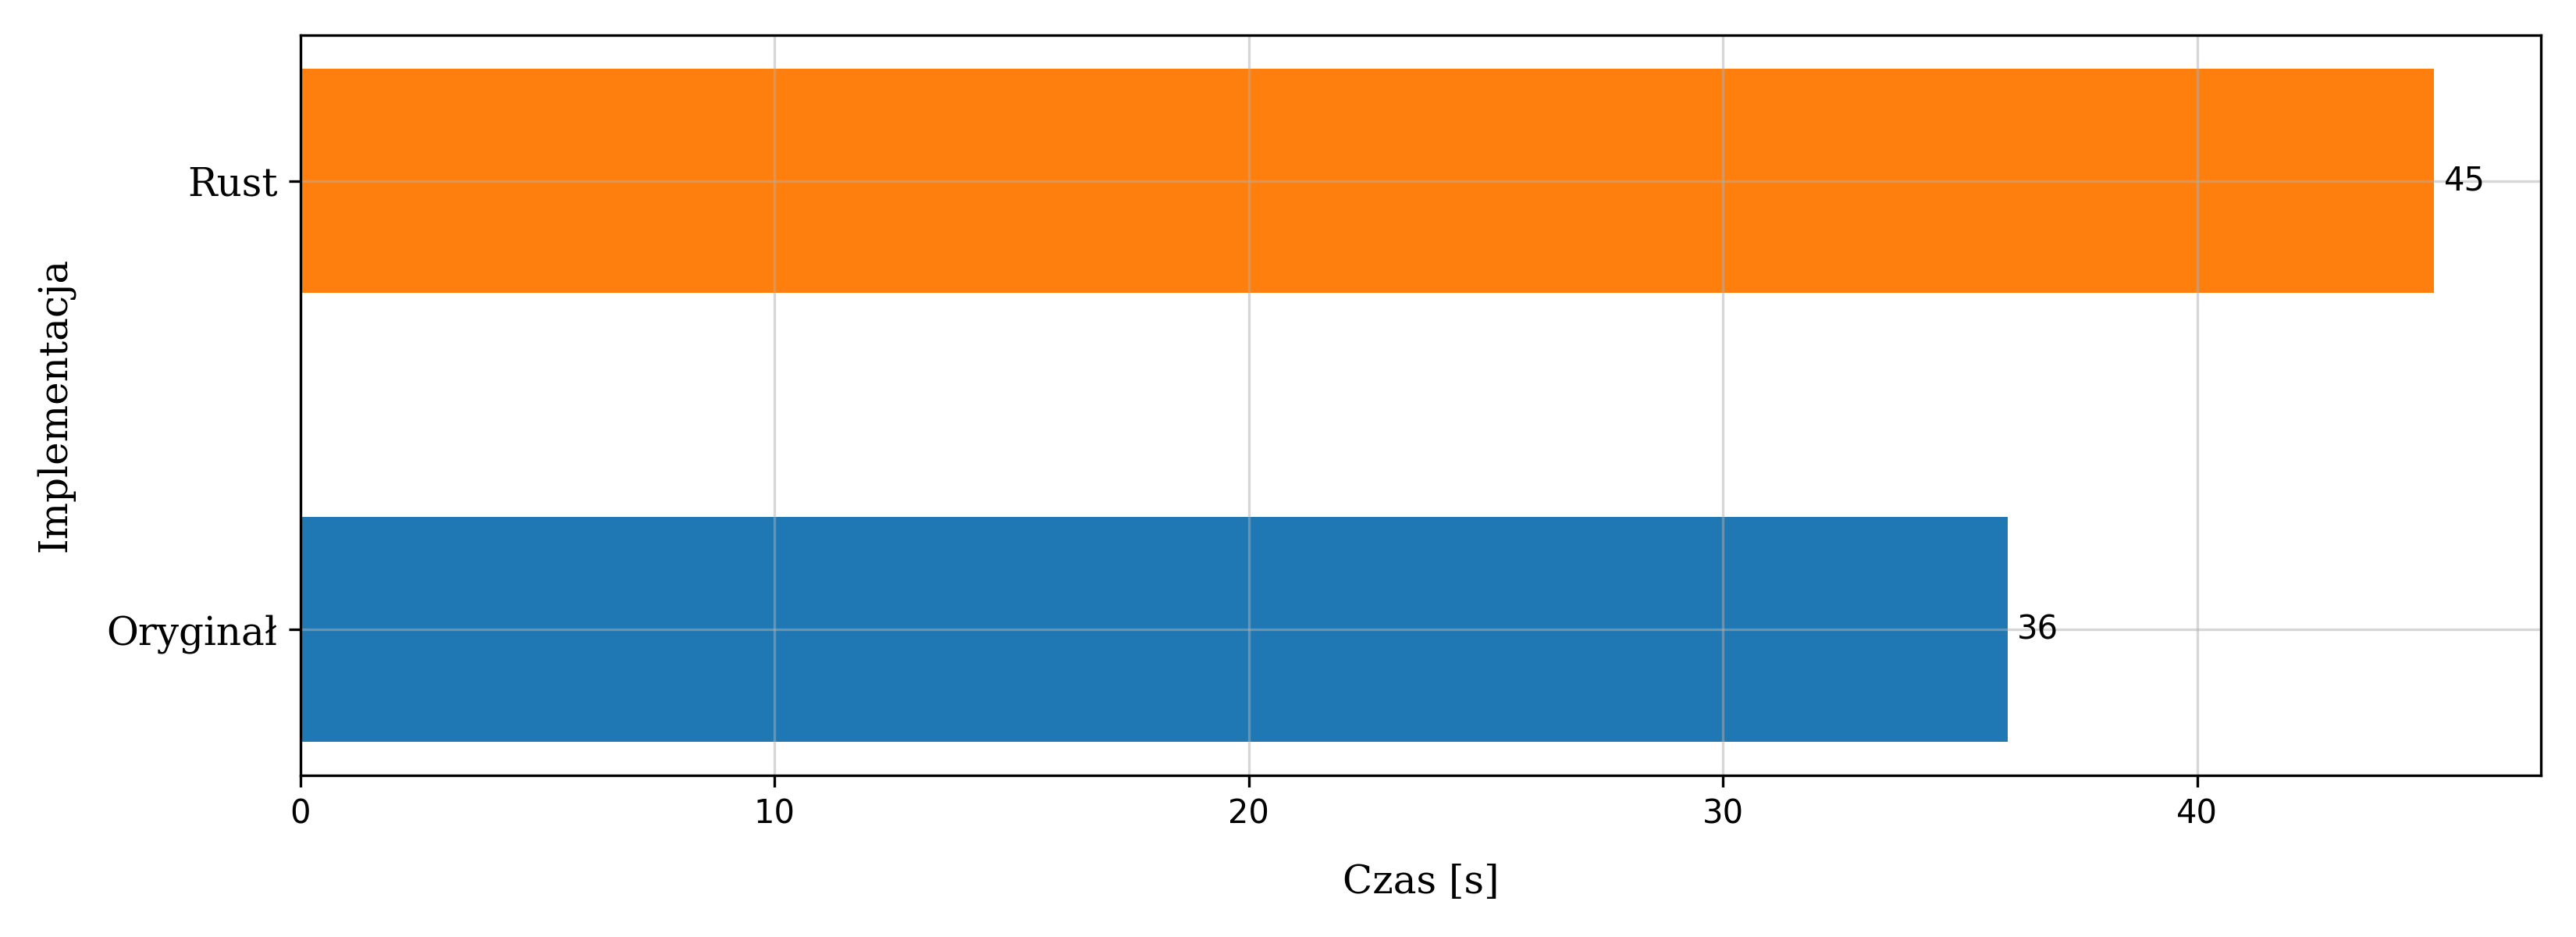
\includegraphics[width=1.0\textwidth]{"resources/benchmark_2/plot2.png"}
      \caption{Wyniki testów wydajności alternatywnej implementacji Python i NumPy (niebieski) w porównaniu do implementacji oryginalnej z zablokowaną ilością wątków (pomarańczowy) dla macierzy $\rho
      _{7}$.}
      \label{first-alt-perf}
    \end{figure}
    \FloatBarrier

    Przekazując do programu macierz $\rho_{0}$, przedstawioną na rysunku \ref{rho-0}, uzyskałem
    wyniki różniące się od tych wykorzystujących macierze $\rho_{2}$ - $\rho_{6}$.
    Wyniki te zostały przedstawione na rysunku \ref{first-alt-perf}, gdzie kolorem pomarańczowym
    oznaczone są wyniki oryginalnej implementacji, natomiast kolorem niebieskim, wyniki nowo
    utworzonego kodu. Na wykresie widoczna jest około 20\% redukcja długości czasu pracy
    przy takich samych danych wejściowych.

    Ponieważ macierz $\rho_{0}$ występuje tylko w jednym rozmiarze, nie jest możliwe aby
    uzyskać tak szerokie spektrum wyników jak w przypadku macierzy $\rho_{2}$ -
    $\rho_{6}$. Z tego względu macierze $\rho_{2}$ - $\rho_{6}$ stanowią wygodny zestaw danych
    do weryfikacji ogólnej charakterystyki zachowania alternatywnych implementacji algorytmu
    i będą dalej wykorzystywane w testach wydajności.

    \newpage


    \subsubsection{ Python i NumPy z AOT }


    Pomiary czasu pracy były wykonywane przy użyciu macierzy $\rho_{2}$ - $\rho_{6}$.
    Dane przekazywałem kolejno do programu z poleceniem działania w trybie FSnQd\footnote{Tryb
    FSnQd jest odpowiednikiem trybu 1 (full separability of an n-quDit state) z oryginalnego
    kodu.} do osiągnięcia co najmniej 1000 korekcji lub do 2.000.000 iteracji algorytmu,
    w zależności od tego co nastąpi szybciej. Dla wszystkich macierzy algorytm uzyskał
    co najmniej 1000 korekcji i w żadnym przypadku nie osiągnął maksymalnej ilości
    iteracji. Dla każdej macierzy pomiar był powtarzany pięciokrotnie a wyniki zostały uśrednione.
    Podczas obliczeń ziarno domyślnego globalnego generatora liczb losowych biblioteki
    NumPy było ustawione na 0. Program działał z zablokowaną ilością wątków
    obliczeniowych. Pomiary czasu pracy dotyczyły przede wszystkim samego algorytmu\footnote{Nie
    biorą więc pod uwagę czasu pochłoniętego przez importowanie modułów itp., natomiast
    operacje wczytywania danych i pisania do plików są wliczane w czas pracy.}.

    \FloatBarrier
    \begin{figure}[ht]
      \centering
      \includegraphics[width=0.9\textwidth]{"resources/benchmark_3/plot.png"}
      \caption{Wyniki testów wydajności alternatywnej implementacji Python i NumPy (niebieski) w porównaniu do implementacji Python i NumPy z AOT (pomarańczowy) dla macierzy $\rho
      _{2}$ - $\rho_{6}$.}
      \label{second-perf}
    \end{figure}
    \FloatBarrier

    W testach nie była widoczna żadna istotna statystyczne zmiana wydajności. Na rysunku
    \ref{second-perf} kolorem pomarańczowym oznaczone zostały czasy pracy implementacji
    z AOT, w zależności od rozmiaru macierzy gęstości. Niebieskie kolumny to czasy pracy
    alternatywnej implementacji bez AOT.

    \subsubsection{ Python i NumPy z JIT }


    \subsubsection{ Rust }


    \subsection{Precyzja obliczeń}


    Oryginalny program posługiwał się liczbami zespolonymi stworzonymi na bazie
    zmiennoprzecinkowych podwójnej precyzji. Jednak w przypadku analizowania niewielkich
    macierzy ponieważ analizowane dane utrzymują zakres wartości blisko 0, do
    efektywnych obliczeń nie jest konieczna podwójna precyzja. Podstawową zaletą tej zmiany
    jest zmniejszenie rozmiaru macierzy w pamięci, a to w pozwala na umieszczenie
    większej części macierzy w pamięci podręcznej procesora. Dodatkowo zwiększa to przepustowość
    wektoryzowanego kodu (Zestawy instrukcji FMA używają rejestrów o rozmiarach 128 i
    256 bit, można więc w jednym takim rejestrze umieścić dwukrotnie więcej 32 bitowych liczb
    pojedynczej precyzji niż 64 bitowych podwójnej).

    \subsection{Pomiary czasu pracy}


    \subsection{Ponowne profilowanie}


    \subsection{Funkcja kronecker}


    \subsection{Funkcja product}


    \section{Wyniki}


    \section{Dyskusja}
  \end{sloppypar}
  \newpage
  \begin{sloppypar}
    \medskip


    \printbibliography
    [heading=bibintoc, title={Odwołania}]
  \end{sloppypar}
\end{document}